%#!platex main

\chapter*{練習問題の解答}

\section*{\ref{134138_29Mar06}章}

\paragraph{\ref{ex:intro01}}

略

\paragraph{\ref{ex:intro02}}

\verb|x, =, 0, ;, while, (, i, <, 100, ), {, x, +=, i, ;, i, ++, ;, }|

\section*{\ref{151253_30Mar06}章}

\paragraph{\ref{ex:cfg_03}}

\begin{center}
 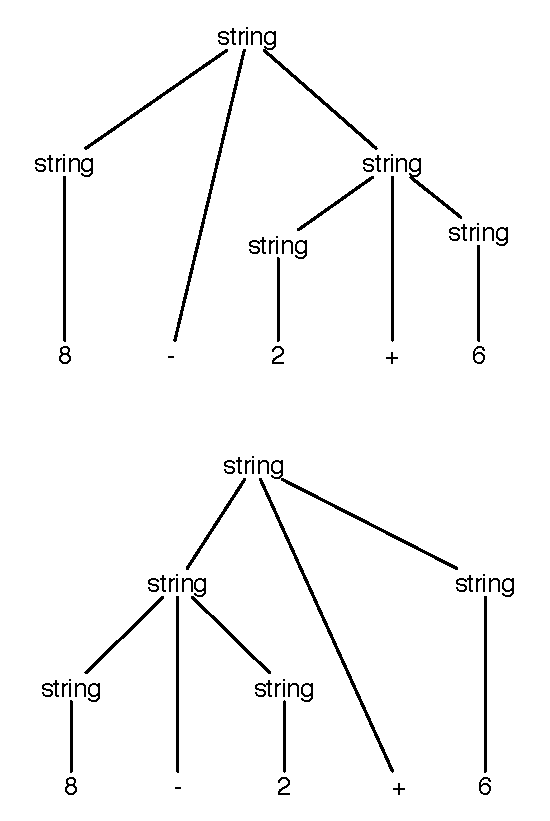
\includegraphics[scale=0.8]{figure/ans_cfg_03.pdf}
\end{center}

$+, -$は左結合の演算子であり、括弧がなければ式の左から計算していく
のが正しい意味になる。したがって、下側の解析木のほうが自然である。
このように、文法によっては、同じ記号列に対して解析木が2通り以上考
えられる場合がある。このような文法を{\bfseries 曖昧である}という。

\paragraph{\ref{ex:cfg_04}}

$0$が$n$個($n \geq 1$)並んだ後に$1$が$n$個並んだような文字列すべて
からなる言語。$0, 1$をそれぞれ$\{, \}$に置き換えてみると、これは対
応関係のとれた括弧の入れ子を表す。この言語は正則言語ではない例とし
て有名である。つまり、この言語は正則表現では書けず、またこの言語を
受理する有限オートマトンも作れない。

\paragraph{\ref{ex:cfg_01}}

\[
 S \Rightarrow A1B \Rightarrow 0A1B \Rightarrow 00A1B \Rightarrow
 001B \Rightarrow 0010B \Rightarrow 00101B \Rightarrow 00101
\]
\[
 S \Rightarrow A1B \Rightarrow A10B \Rightarrow A101B \Rightarrow
 A101 \Rightarrow 0A101 \Rightarrow 00A101 \Rightarrow 00101
\]

\paragraph{\ref{ex:cfg_02}}

\begin{eqnarray*}
 E & \rightarrow & TE' \\
 E' & \rightarrow & + TE' \mid \epsilon \\
 T & \rightarrow & FT' \\
 T' & \rightarrow & * FT' \mid \epsilon \\
 F & \rightarrow & (E) \mid \mathbf{id}
\end{eqnarray*}
